\documentclass[10pt, handout, xcolor=table]{beamer}

\usepackage[utf8]{inputenc}
\usepackage{amsmath}
\usepackage{amsfonts}
\usepackage{amssymb}
\newcommand*\themecol{\usebeamercolor[fg]{structure}}

\setbeamertemplate{navigation symbols}{}
 \setbeamertemplate{footline}[frame number]

\newcommand{\overbar}[1]{\mkern 1.5mu\overline{\mkern-1.5mu#1\mkern-1.5mu}\mkern 1.5mu}

\usepackage{tikz}
\usetikzlibrary{shapes.geometric, arrows}
\tikzstyle{prob} = [rectangle, minimum width=3cm, text width = 4.5cm, minimum height=1cm, text centered, draw=black, fill= blue!20]
\tikzstyle{stat} = [rectangle, minimum width=3cm,  text width = 4.5cm, minimum height=1cm, text centered, draw=black, fill= red!20]
\tikzstyle{arrow} = [thick,->,>=stealth]


\setlength{\parindent}{0pt}
\setlength{\parskip}{6pt}

\title{STAT 111\\
{\small Recitation 3}}

\author{Mo Huang}
\institute{Email: mohuang@wharton.upenn.edu \\
\vspace{0.25cm}
Office Hours: Wednesdays 3:00 - 4:00 pm, JMHH F96\\
\vspace{0.25cm}
Slides (adapted from Gemma Moran): \url{github.com/mohuangx/STAT111-Fall2018} }


\date{September 21, 2018}


\begin{document}

\begin{frame}
\titlepage
\end{frame}


\begin{frame}{Random Variables: Mean}
\begin{itemize}
\setlength{\itemsep}{15pt}
\item<1-> The {\themecol mean of a random variable} (expected value) is the long-run average of realizations of the random variable over repeated experiments.
\item<2-> This mean of random variable $X$ is different from the sample average, which is the average of a \emph{finite} number of observations ($\overbar{x} = \frac{x_1 + x+2 + \cdots + x_n}{n}$, where $x_1, \ldots, x_n$ are observed data).
\item<3-> Let $X$ be a discrete random variable that can take values $\{v_1,v_2,\dots, v_k\}$. Then the mean of $X$ is given by:
\begin{align*} 
\mu &= \sum_{i = 1}^k v_i P(X = v_i)\\
&= v_1P(X = v_1) + v_2P(X = v_2) + \cdots + v_kP(X = v_k).
\end{align*}
\item<4-> If $X$ is binomial with parameters $n$ and $\theta$, then the mean of $X$ is 
\[\mu = n \theta\]
\end{itemize}
\end{frame}



\begin{frame}{Random Variables: Variance}

\begin{itemize}
\setlength{\itemsep}{15pt}
\item<1-> The {\themecol variance of a random variable} is a measure of the \emph{spread} of a distribution - that is, how far away values are from the mean.
\item<2-> Let $X$ be a discrete random variable that can take values $\{v_1,v_2,\dots, v_k\}$. Then the variance of $X$ is given by:
\begin{align} 
\sigma^2 &= (v_1 - \mu)^2P(X = v_1) + \cdots + (v_k - \mu)^2P(X = v_k) \\
&\hspace{3cm} \text{\themecol\emph{or} } \notag\\
\sigma^2&= v_1^2P(X=v_1) + \cdots + v_k^2P(X = v_k) - \mu^2
\end{align} 
\item<3-> The {\themecol standard deviation of a random variable} is the square root of the variance and is denoted by $\sigma$.
\item<4-> For a {\themecol binomial }random variable $X\sim \mathcal{B}(n, \theta)$:
$$\sigma^2 = n\theta(1-\theta)$$
\end{itemize}

\end{frame}

\begin{frame}{Random Variables: Questions}
\begin{itemize} 
\item[Q1:] Let $X$ be a random variable with the below distribution. Find the mean and the variance of $X$ using formula (1) and then formula (2).
\begin{table}
\begin{tabular}{|c|c|c|c|c|}
\hline
\rowcolor{blue!10} $x$ & -3 & -1 & 4&5  \\ \hline
$P(X = x)$ & 0.1 & 0.3 & 0.4 &0.2 \\
\hline
\end{tabular}
\caption{Probability distribution of $X$.} 
\end{table}
\item<2->[A1:]  {\color{red} $\mu = -3\times 0.1 -1\times 0.3 + 4\times 0.4 + 5\times 0.2 =2.$
\begin{align*}
\sigma^2&= (-3-2)^2(0.1) + (-1-2)^2(0.3) + (4-2)^2(0.4) + (5-2)^2(0.2) \\
&= 8.6.\\
  \\
\sigma^2 &= (-3)^2(0.1) + (-1)^2(0.3) + 4^2(0.4) + 5^2(0.2) - 2^2\\
&=8.6.
\end{align*}}
\end{itemize} 

\end{frame}

\begin{frame}{Random Variables: Questions}
\begin{itemize} 
\item[Q2:] Let $X$ be a random variable with the below distribution. Write the probability distribution of $Y = 2X$ in tableau form.
\bigskip
\begin{table}
\begin{tabular}{|c|c|c|c|c|}
\hline
\rowcolor{blue!10} $x$ & -3 & -1 & 4&5  \\ \hline
$P(X = x)$ & 0.1 & 0.3 & 0.4 &0.2 \\
\hline
\end{tabular}
\caption{Probability distribution of $X$.} 
\end{table}
\item<2->[A2:]  {\color{red} Probability distribution of $Y$:}
\bigskip
\begin{table}[H]
\begin{tabular}{|c|c|c|c|c|}
\hline
\rowcolor{blue!10} $y$ & -6 & -2 & 8 & 10  \\ \hline
$P(Y = y)$ & 0.1 & 0.3 & 0.4 &0.2 \\
\hline
\end{tabular}
\caption{Probability distribution of $Y$.} 
\end{table}
\end{itemize} 

\end{frame}


\begin{frame}{Properties of mean and variance}

\begin{itemize}\itemsep3ex
\item<1-> Suppose $X$ is a random variable with mean $\mu$ and variance $\sigma^2$. Consider fixed number $c$.
\item<2-> Mean properties
\begin{itemize}
\item<2-> Mean of $X + c \Longrightarrow \mu + c$.
\item<2-> Mean of $cX \Longrightarrow c\mu$.
\end{itemize}
\item<3-> Variance properties
\begin{itemize}
\item<3-> Variance of $X+c \Longrightarrow \sigma^2$.
\item<3-> Variance of $cX \Longrightarrow c^2 \sigma^2$.
\end{itemize}
\item<4->[Q3:] Suppose $X$ has mean $\mu_X = 3$ and variance $\sigma^2_X = 4$. What is the mean and variance of $Y = 2+5X$?
\item<5->[A3:] {\color{red} $\mu_Y = 2+5\mu_X = 2+5(3) = 17$\\
\medskip
$\sigma^2_Y = 5^2 \sigma^2_X = 5^2(4) = 100$
}
\end{itemize}

\end{frame}

\begin{frame}{Many Random Variables}
\begin{itemize}
\setlength{\itemsep}{15pt}
\item<1-> Suppose we plan an experiment with a {\themecol sample size} of $n$. 
\item<2-> We have $n$ future outcomes, or random variables, denoted by: $X_1, X_2, \dots, X_n$.
\item<3-> We say $\{X_1,\dots, X_n\}$ are {\themecol independently and identically distributed (or i.i.d)} if:
\begin{itemize}
\setlength{\itemsep}{10pt}
\vspace{0.25cm}
\item All the $X_i$s are independent of each other.
\item Each $X_i$ has the same probability distribution.
\end{itemize}
\item<4-> For example:
\begin{itemize}
\item \color{blue!70} I plan to roll a dice $n$ times. $X_i$ represents the future outcome of the $i$th roll. $X_i$ is \emph{independent} of the other rolls of the dice, and it has the same probability of getting a $1, 2, 3, 4, 5, 6$ as the other rolls.
\end{itemize}
\end{itemize}
\end{frame}


\begin{frame}{Many Random Variables}
\begin{itemize}
\setlength{\itemsep}{15pt}
\item<1-> Recall the sample average is given by:
\begin{align*}
\bar{x} = \frac{x_1 + \cdots + x_n}{n}.
\end{align*} 
\item<2-> What if we haven't observed the data $x_1,\dots, x_n$ yet?
\item<3->  Before an experiment, the average is \emph{also} a random variable:
\begin{align*}
\bar{X} = \frac{X_1 + \cdots + X_n}{n}
\end{align*}
\item<4-> The \emph{sum} is also a random variable:
\begin{align*}
T_n = X_1 + \cdots + X_n
\end{align*}
\end{itemize}
\end{frame}

\begin{frame}{Many Random Variables}
\begin{itemize}
\setlength{\itemsep}{15pt}
\item<1-> Let $X$ and $Y$ be two random variables. Then,
\vspace{0.25cm}
\begin{itemize}
\setlength{\itemsep}{10pt}
\item[]<2-> {\color{blue}$\text{mean}(X + Y) = \text{mean}(X) + \text{mean}(Y).$} 
\item<3-> If $X$, $Y$ are also independent,
\item<3->[] {\color{blue}$\text{variance}(X +Y) = \text{variance}(X) + \text{variance}(Y).$}
\item<4-> For constants $a, b$, we have
\item<4->[] {\color{blue}$\text{mean}(aX + bY) = a\times \text{mean}(X) + b\times\text{mean}(Y)$}
\item<4->[] {\color{blue}$\text{variance}(aX + bY) = a^2\times\text{variance}(X) + b^2\times\text{variance}(Y).$}
\end{itemize}
\item<5-> Let $D = X - Y$. What is the variance of $D$?
\item<6->[] \color{blue}$\text{variance}(D) = \text{variance}(X) {\color{red}  +  } \text{variance}(Y)$.
\end{itemize}
\end{frame}

\begin{frame}{Many Random Variables}

\begin{itemize}
\setlength{\itemsep}{15pt}
\item Let $X_1, \dots, X_n$ be i.i.d. random variables, each with mean $\mu$ and variance $\sigma^2$.
\item Then for the sum, $T_n$:
$${\color{blue}\text{mean of }T_n = n\mu, \quad \text{variance of }T_n = n\sigma^2}$$
\item For the average, $\bar{X}$:
$${\color{blue} \text{mean of }\bar{X} = \mu, \quad \text{variance of } \bar{X} = \frac{\sigma^2}{n}.}$$
\end{itemize}

\end{frame}

\begin{frame}{Questions}
\begin{itemize}
\setlength{\itemsep}{15pt}
\item[Q4:] Suppose we have a company producing a medicine. Each day the \emph{mean} amount of medicine produced is 500 mg and the \emph{variance} is 900 mg$^2$. Assume the amount produced each day is independent.
\item[(i)] Let $T_n$ be the total amount of medicine produced in a week. Find the mean and variance of $T_n$. 
\item<2->[] {\color{red} $Mean(T_n) =   5\times 500 = 2500$}

 {\color{red} $Var(T_n) = 5\times 900 = 4500$}
\item<3->[(ii)] Let $\bar{X}$ be the average amount of medicine produced in a 5-day week. Find the mean and variance of $\bar{X}$.
\item<4->[] {\color{red} $Mean(\bar{X}) = 500$} 

{\color{red} $Var(\bar{X}) = 900/5 = 180$}
\end{itemize}
\end{frame}

\begin{frame}{Proportions}

\begin{itemize}
\setlength{\itemsep}{15pt}
\item<1-> Sometimes it is necessary to consider the \emph{proportion} of ``successes'' in a Binomial trial (instead of the total number of successes)
\item<2-> Proportions are a type of average!
\item<3-> Let 
\begin{align*}
Y_i = 
\begin{cases}
1 &\text{if the }i\text{th trial is a ``success''}\\
0 &\text{if the }i\text{th trial is a ``failure''}
\end{cases}
\end{align*}
\item<4-> Then we have $Y_1,\dots, Y_n$ where $Y_i\sim Binomial(1,\theta)$.
\item<5-> The proportion of successes is the average:
\begin{align*}
P = \frac{Y_1 + \dots + Y_n}{n}
\end{align*}
\end{itemize}
\end{frame}

\begin{frame}{Proportions}
\begin{itemize}
\setlength{\itemsep}{-5pt}
\item<1-> $Y_i \sim Binomial(1,\theta)$. Recall: 
$$\color{blue} Mean(Y_i) = \theta, \quad Var(Y_i) = \theta(1-\theta).$$
\item<2-> The proportion of successes is the average:
\begin{align*}
P = \frac{Y_1 + \dots + Y_n}{n}
\end{align*}
\item<3-> Then, 
$$\color{blue} Mean(P) = \theta, \quad Var(P) = \frac{\theta(1-\theta)}{n}$$.
\vspace{0.5cm}
\item<4->[Q5:] Suppose we plan to toss a coin 20 times and $Prob(H) = 0.7$. Let $P$ be the \emph{proportion} of heads that we toss. Find the mean and variance of $P$.
\vspace{0.25cm}
\item<5->[A5:] 
 $$\color{red}Mean(P) = 0.7, \quad Var(P) = 0.7\times 0.3 / 20 = 0.0105.$$
\end{itemize}
\end{frame}


\begin{frame}{Questions}
\begin{itemize}
\setlength{\itemsep}{10pt}
\item<1->[Q6:] Suppose the company producing a medicine has different means and variances the amount produced on each day of the week:
\begin{table}
\begin{tabular}{l|ll}
Day & Mean & Variance \\ \hline
Monday $(X_1)$ & 450 & 1200 \\
Tuesday $(X_2)$ & 550 & 800 \\
Wednesday $(X_3)$ & 600 & 500  \\
Thursday $(X_4)$ & 550 & 800 \\
Friday $(X_5)$ & 350 & 1200 
\end{tabular}
\end{table}
\item<2->[] Find mean and variance of both the sum $T_n$ and the average $\bar{X}$.
\item<3->[A6:] {\color{red} $X_1, X_2, X_3, X_4$, and $X_5$ are no longer $i.i.d.$!\\
\bigskip
$Mean(T_n) = 450 + 550 + 600 + 550 + 350 = 2500$

$Var(T_n) = 1200 + 800 + 500 + 800 + 1200 = 4500$}
\item<4->[] {\color{red} $Mean(\bar{X}) = 1/n \times Mean(T_n) = 500$ 

$Var(\bar{X}) = 1/n^2 \times Var(T_n) = 4500/25 = 180$}
\end{itemize}
\end{frame}

\begin{frame}{Questions}
\begin{itemize}
\setlength{\itemsep}{15pt}
\item<1->[Q7:] Let $P_1$ be the proportion of heads in 50 coin tosses, where $P(H) = 0.6$. Find $Mean(P_1)$ and $Var(P_1)$.
\item<2->[A7:] {\color{red} $Mean(P_1) = 0.6$ and $Var(P_1) = 0.6 \times 0.4/ 50 = 0.0048$.}
\item<3->[Q8:] Let $P_2$ be the proportion of heads in 20 coin tosses, where $P(H) = 0.7$. From earlier, $Mean(P_2) = 0.7$ and $Var(P_2) = 0.0105$. Let $D = P_1 - P_2$. Find the mean and variance of $D$.
\item<4->[A8:] {\color{red} $Mean(D) = 0.6 - 0.7 = -0.1$

$Var(D) = 0.0048 + 0.0105 = 0.0153$}
\end{itemize}
\end{frame}

\begin{frame}{Continuous Random Variables}
\begin{itemize}
\setlength{\itemsep}{10pt}
\item So far, we have just considered discrete random variables; those whose possible values are countable.
\item A {\themecol continuous random variable} can take continuous values in a future experiment.
\item Every continuous random variable $X$ has an associated {\themecol density function} $f(x)$. 
\end{itemize}
\begin{figure}
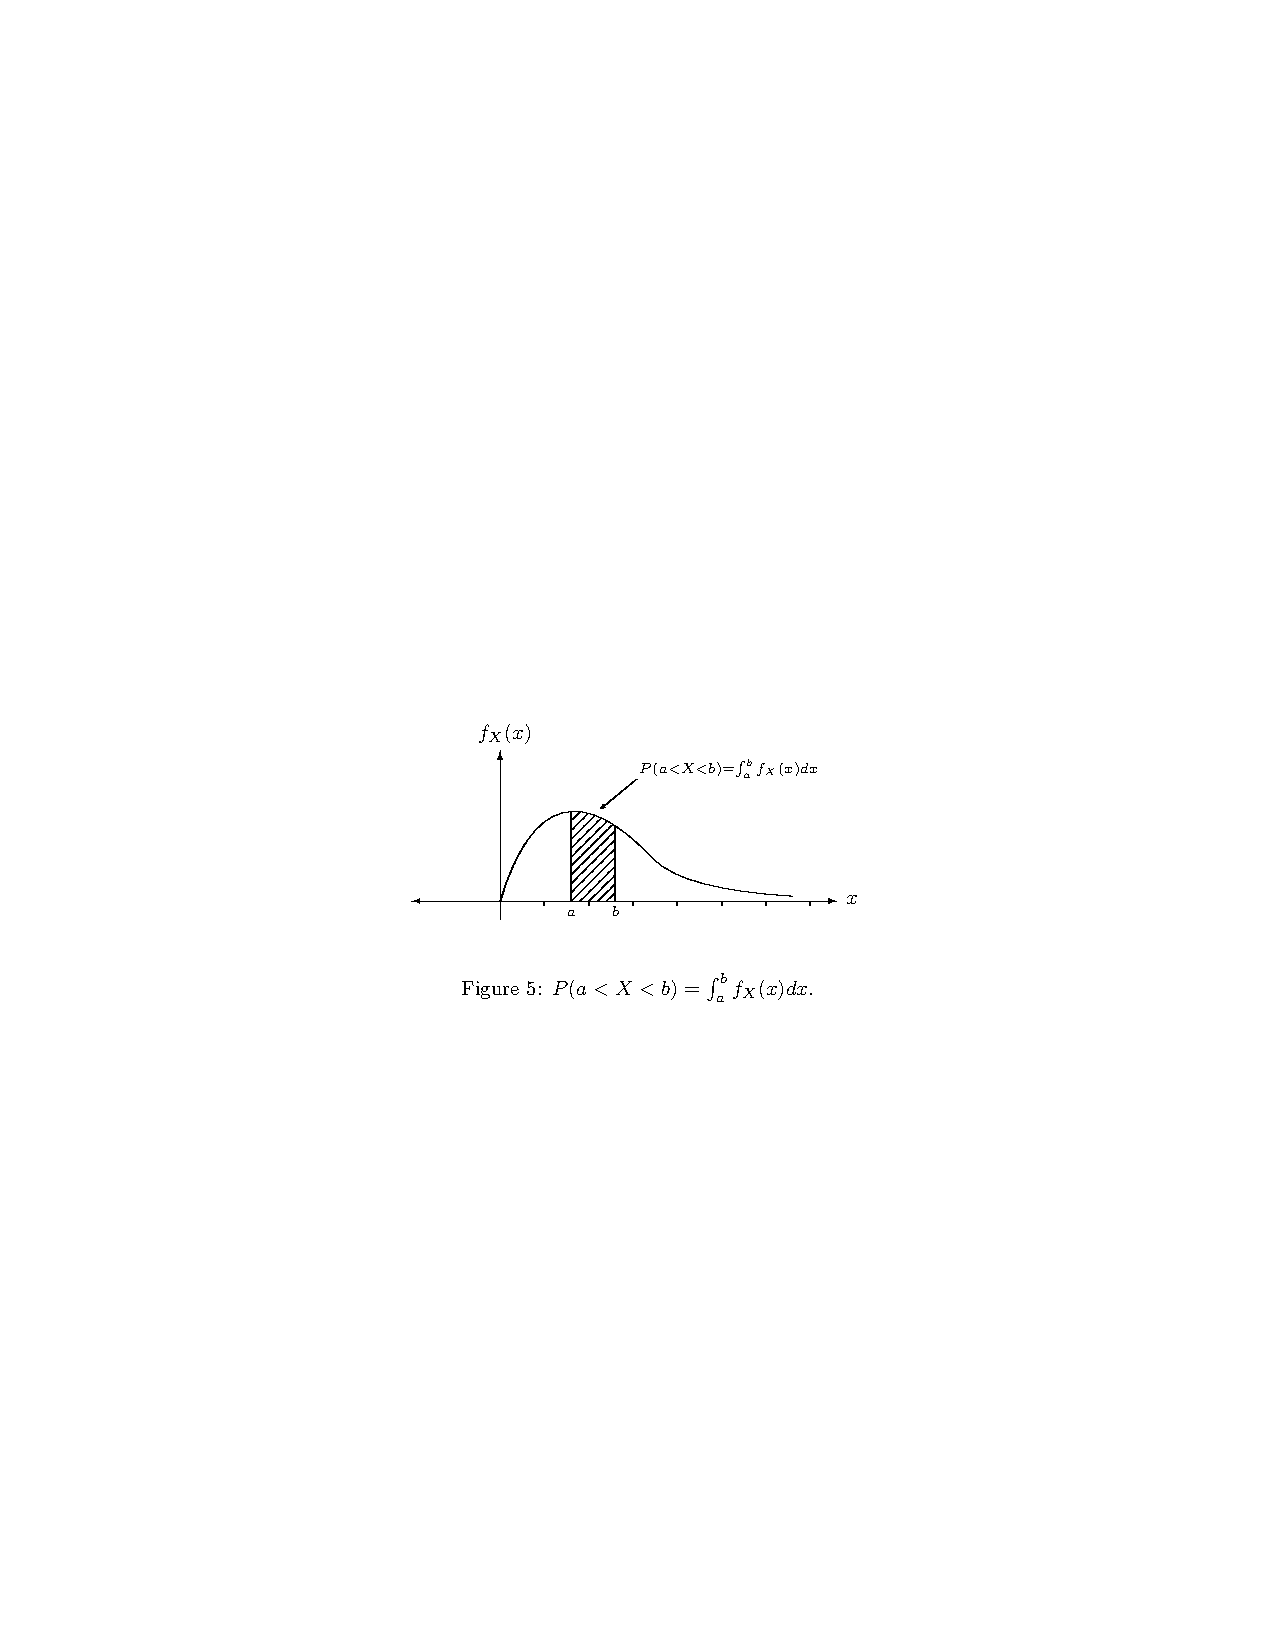
\includegraphics[width = 0.6\textwidth]{images/rec5_1}
\end{figure}
\end{frame}


\begin{frame}{The Normal Distribution}
\begin{itemize}
\setlength{\itemsep}{10pt}
\item A {\themecol normal} random variable is a continuous random variable.
\begin{figure}
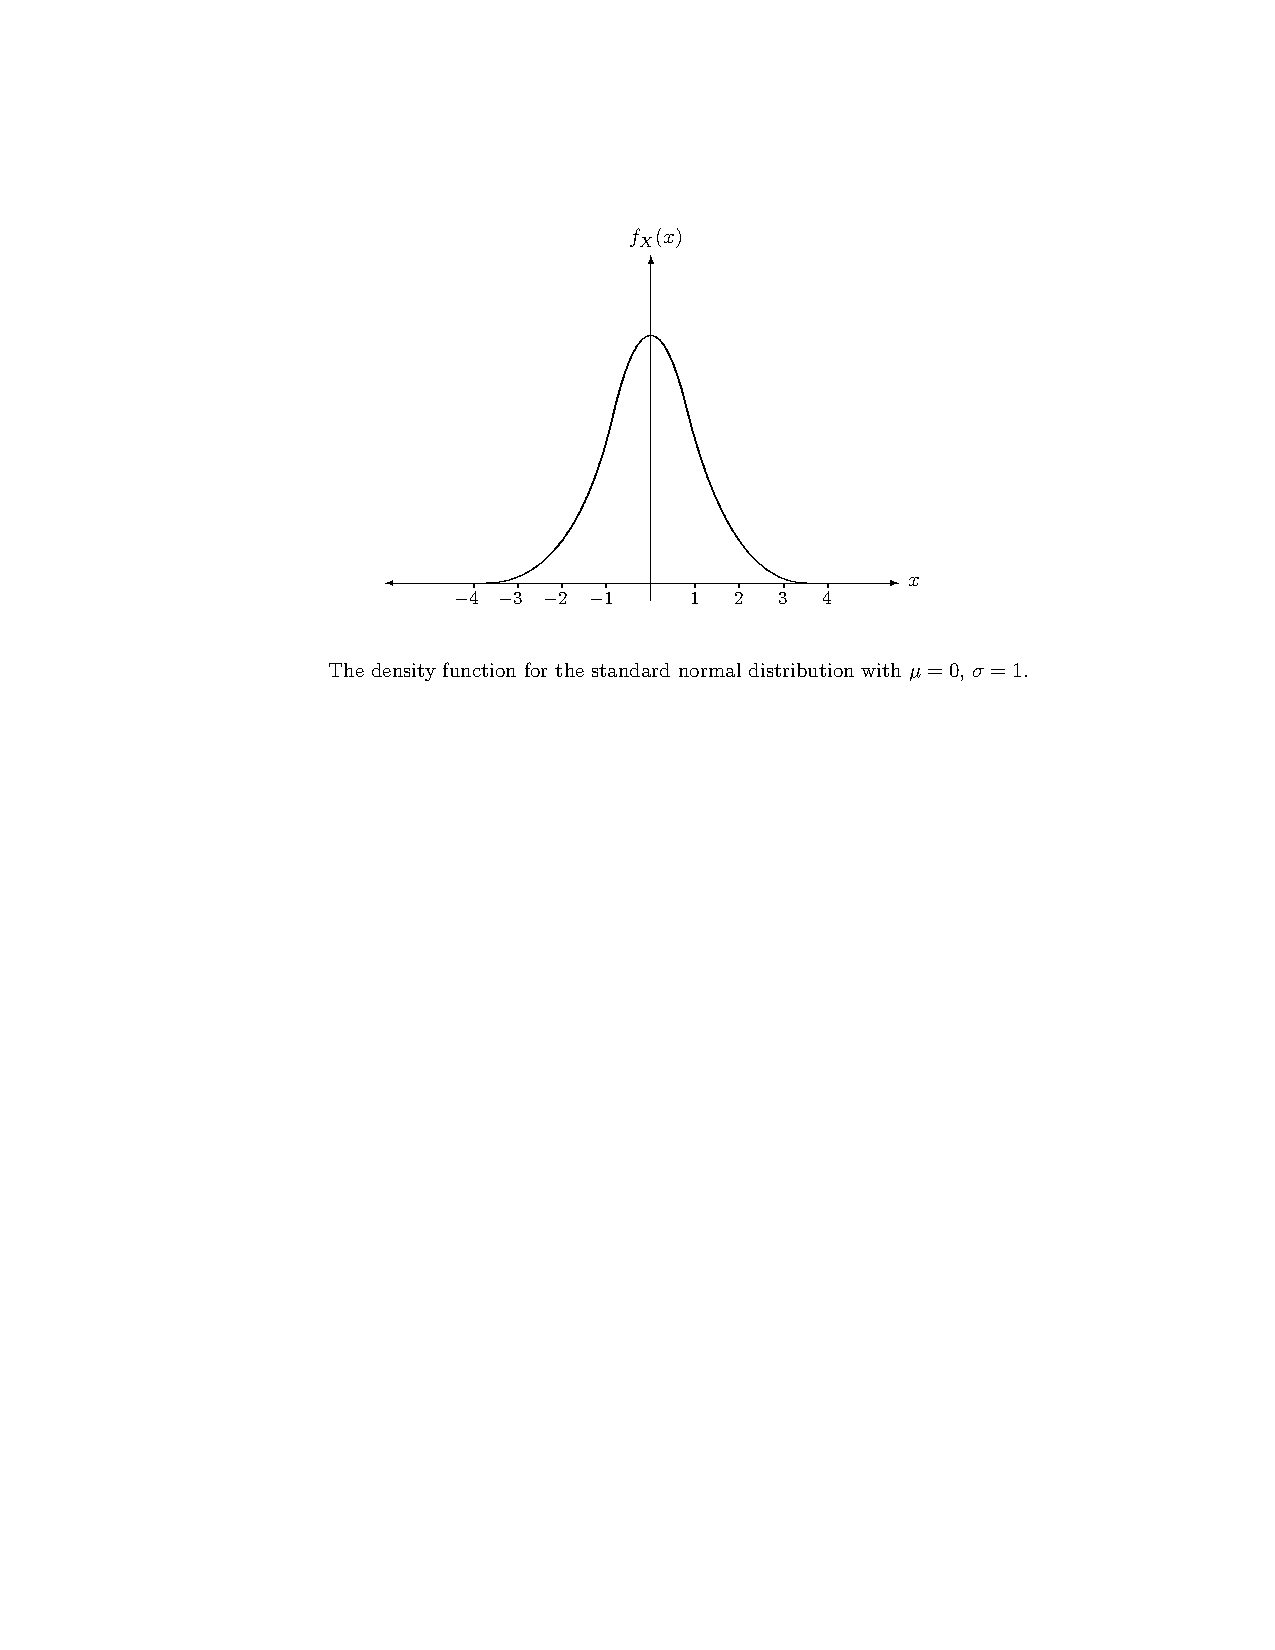
\includegraphics[width = 0.6\textwidth]{images/rec5_2}
\end{figure}
\item We call a normal random variable with $\mu = 0$ and $\sigma^2 = 1$ a {\themecol standard normal} random variable.
\item For standard normal random variables, we can use charts (or a computer) to find the area under the density function (i.e. the probabilities).
\end{itemize}
\end{frame}

\begin{frame}{Questions}
\begin{itemize}
\setlength{\itemsep}{15pt}
\item<1-> $P(Z < -1.75) $ 
\item<2->[] {\color{red}$P(Z < -1.75)= 0.0401$}
\item<3-> $P(Z > 0.85)$ 
\item<4->[]  {\color{red}$P(Z > 0.85)= 1- 0.8023 = 0.1977$}
\item<5->$ P(-1.43 < Z < 0.92) $
\item<6->[]  {\color{red}$P(-1.43 < Z < 0.92)  = 0.8212 - .0764 = .7448$}
\end{itemize}

\end{frame}



\end{document}


